\documentclass[10pt,twocolumn]{article}
\usepackage{amsmath}
\usepackage{graphicx}
\usepackage{mathtools}
\usepackage{fullpage}
\usepackage{float}
\usepackage{color, soul}

\begin{document}
\title{6.867: Homework 1}

\section{Gradient Descent}
Gradient descent works by updating an initial guess by taking a step opposite the direction of the gradient at that initial guess. Moving opposite the gradient helps  to effectively move "downhill" in terms of the function value.  The formulation of the gradient descent method is as follows
\begin{equation}
x(\tau+1) = x(\tau) - \alpha \nabla F(x(\tau))
\end{equation}

Where $ x(\tau)$ is the current guess, with $\tau$ being the current iteration, $\alpha$ is the step size and $F(x)$ is the function which will be evaluated. This method is carried out until there is convergence, which is checked by looking at the norm of successive guesses and seeing if it is less than the required tolerance, $\epsilon$,   



\begin{equation} 
\left \lVert x(\tau+1)-x(\tau) \right \rVert \leq \epsilon
\end{equation}

This is implemented in the code, $grad\_descent.m$ which takes arguments, $x_i, \alpha, \epsilon, f,$ and $df$ where $f$, and $df$ are function handles and returns $x_{min}, f(x_{min})$



\subsection*{ Gradient Descent Testing}

We implemented this code on a few different functions, first simply a 1-D quadratic bowl, then on a N-D quadratic bowl. In these instances the gradient descent performed well, finding the true solution with ease.  
\begin{figure}[H]
\center
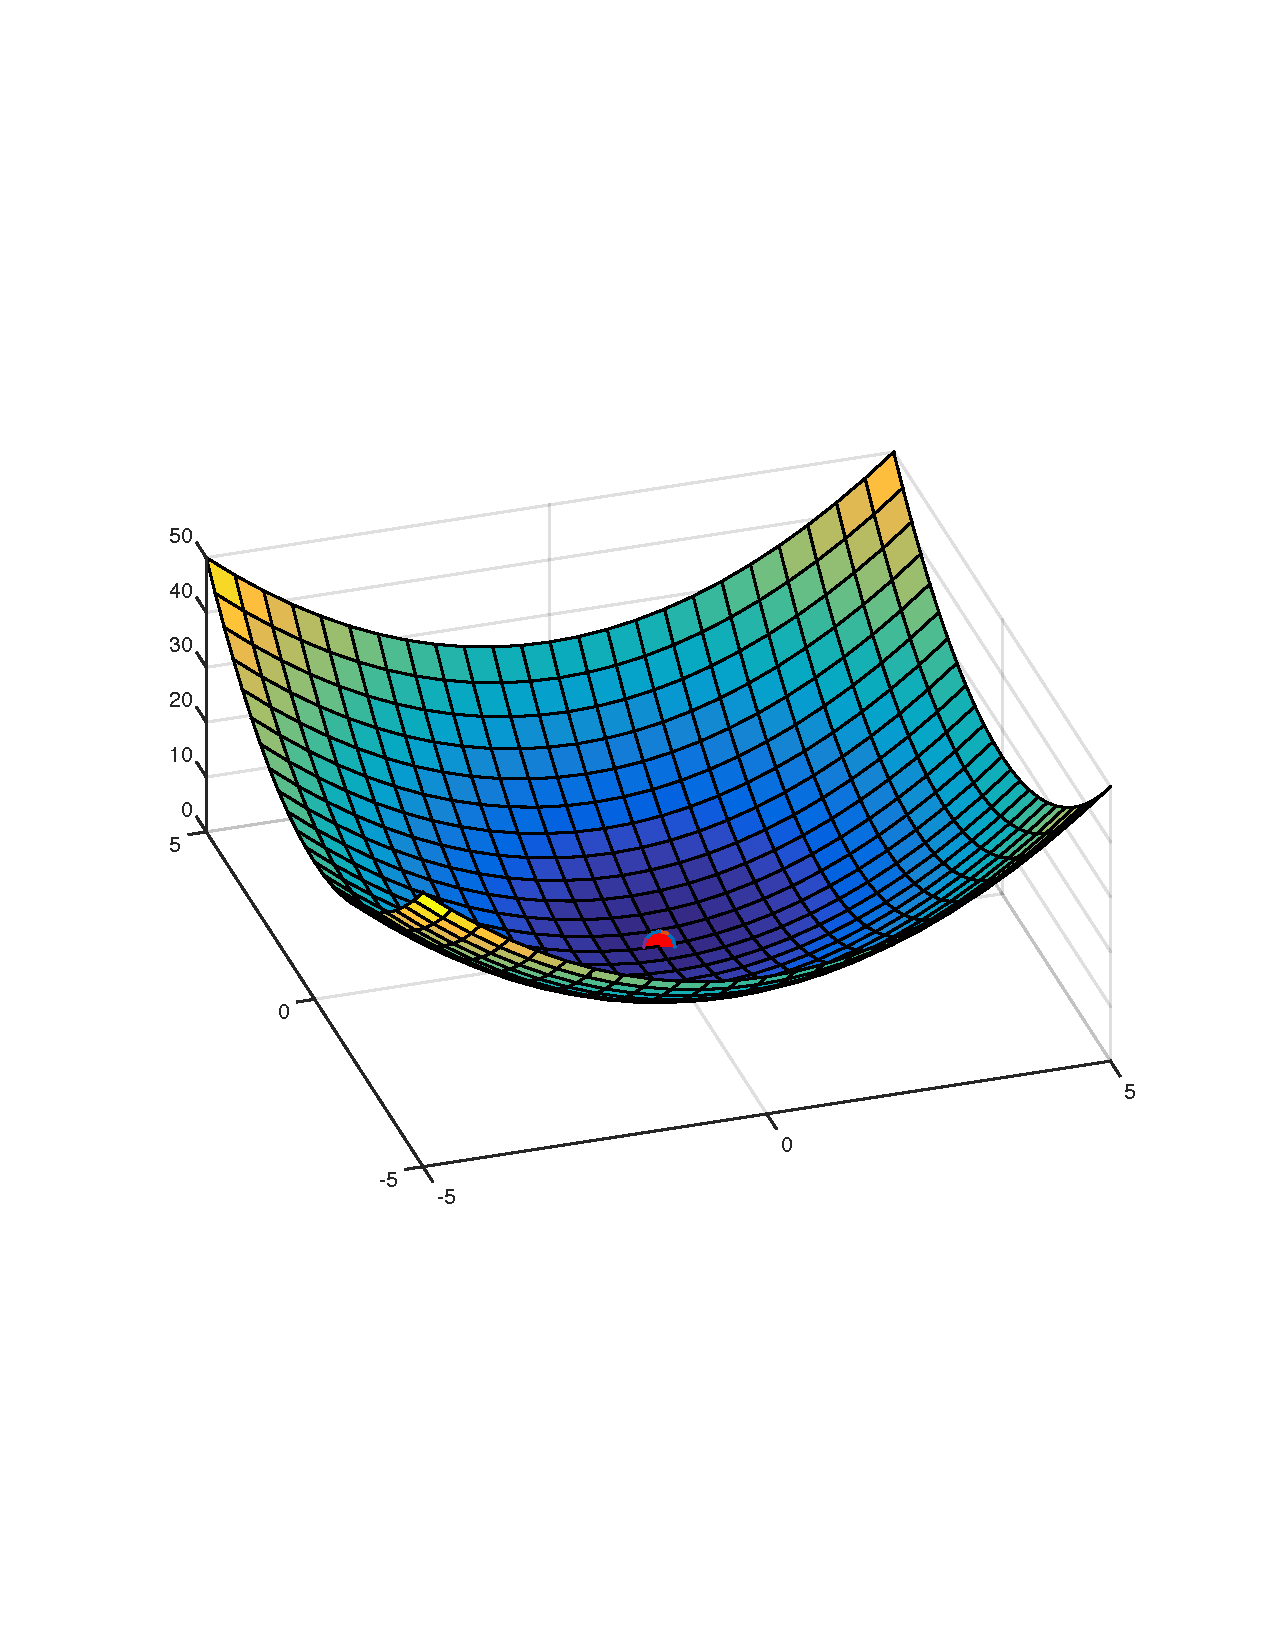
\includegraphics[scale =.4]{2DQuadBowl.pdf}
\caption{Gradient Descent Program located the minimum, indicated by the red dot, on 2D quadratic Bowl}
\end{figure}


By implementing the gradient descent code on a sine wave, which has multiple minima, the effects of input parameters on the declared minima could be investigated. The figures below show the effect of changing the initial guess and the tolerance. 
\begin{figure}[H]
\begin{minipage}{.17\textwidth}
\center
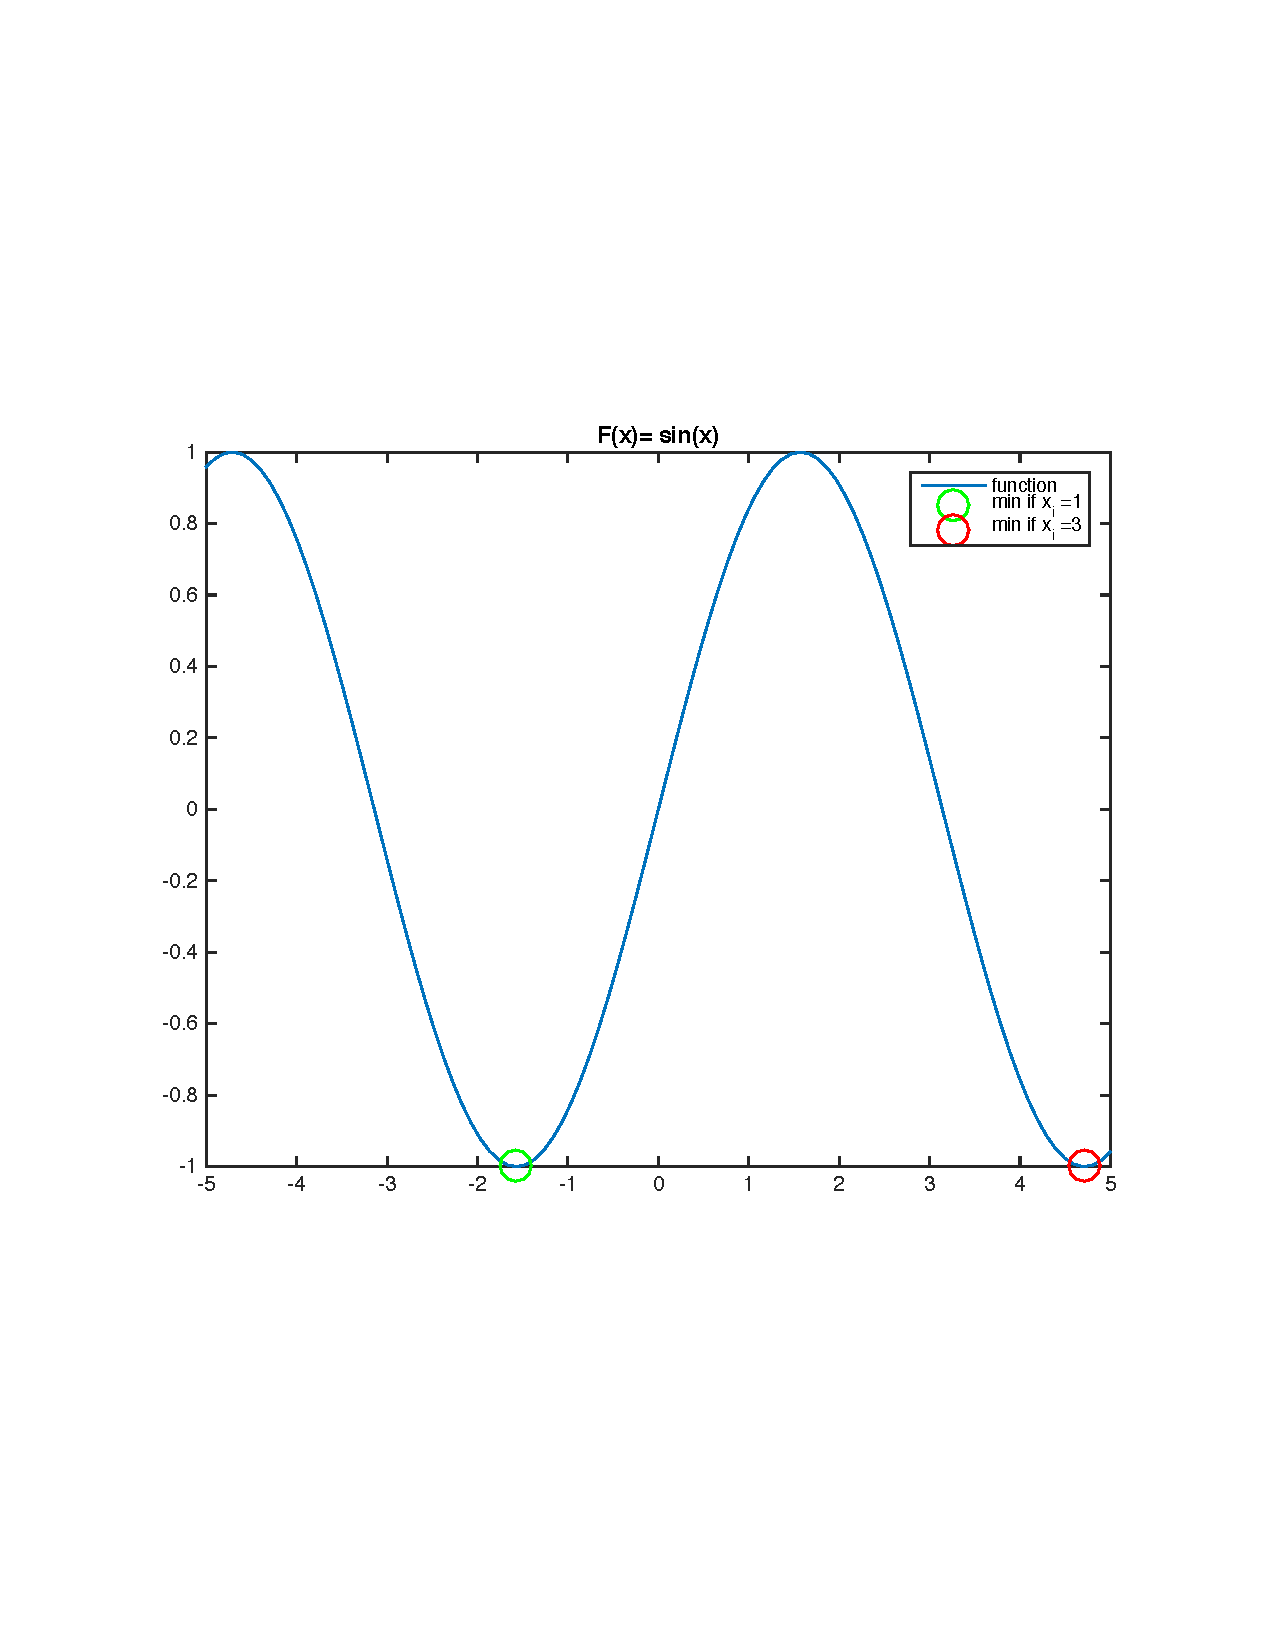
\includegraphics[scale=.17]{1Dsin.pdf}
	
\end{minipage}
\begin{minipage}{.17\textwidth}
\center
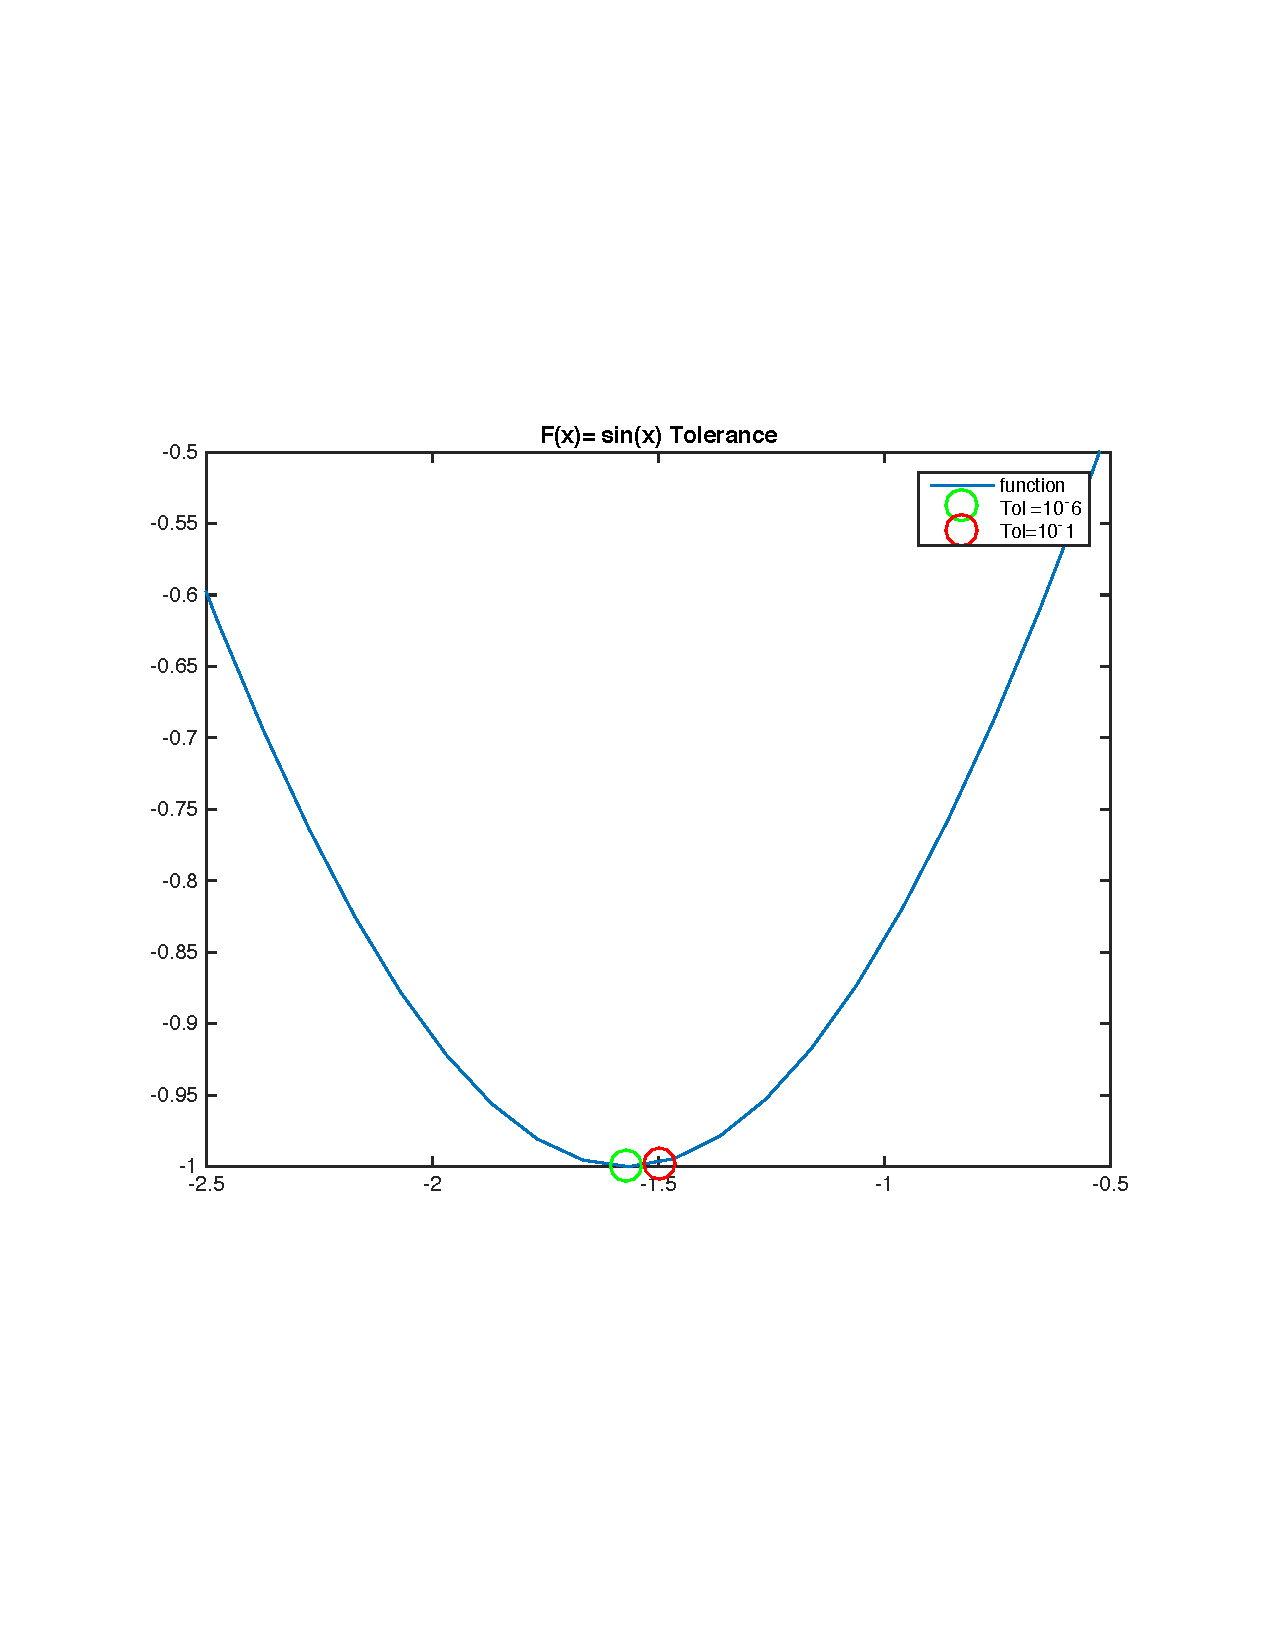
\includegraphics[scale=.17]{1DsinHighTol.pdf}
	
\end{minipage}
\begin{minipage}{.1\textwidth}
\center
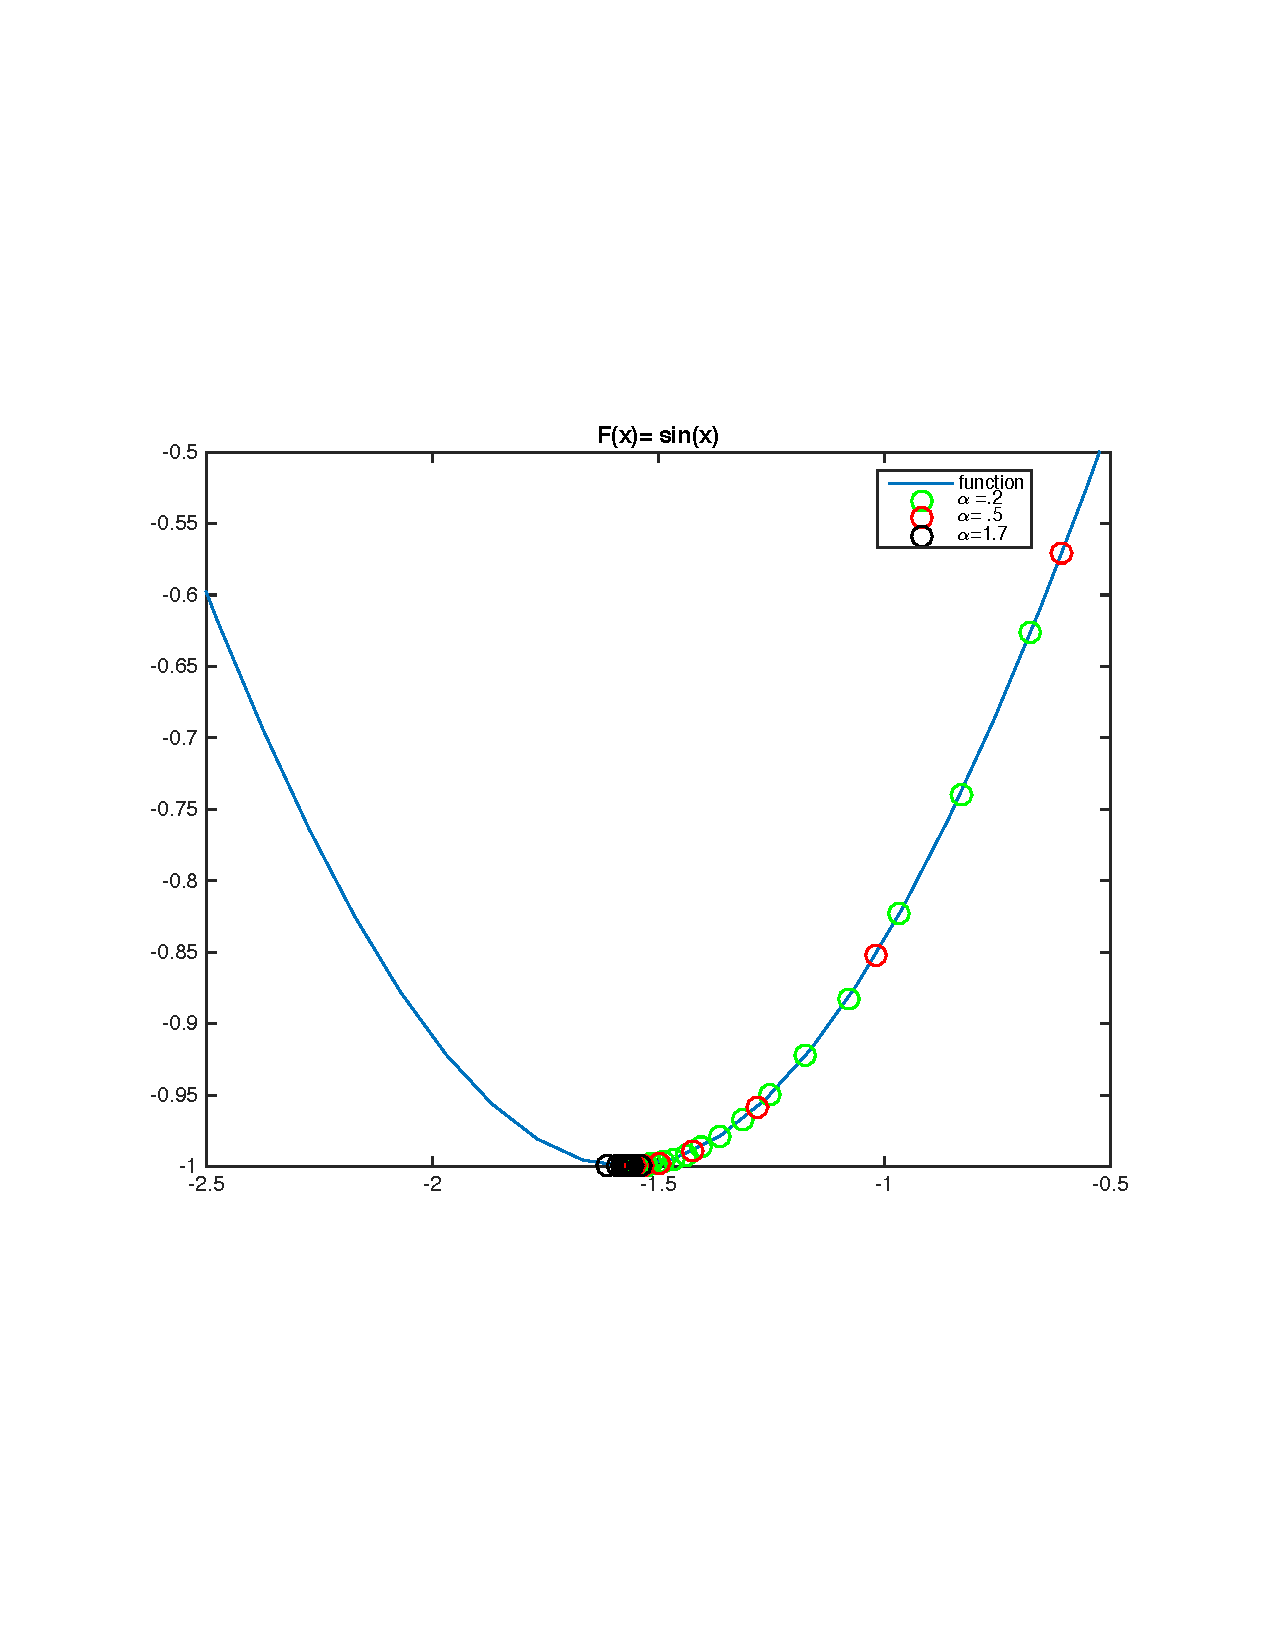
\includegraphics[scale=.17]{1DsinStepSize.pdf}
\end{minipage}
\caption{ Effect of changing input parameters. a) shows the effect of different initial guess leads to a different minimum. b) Setting tolerances too large does not capture true minimum. c) Setting step size too small increases number of iterations. Setting it too large also increases number of iterations by overshooting the minimum}
\end{figure}
By changing the initial guess at points where the slopes head towards different minima of course changes the output of the gradient descent process. If the tolerance is too high, the solver converges too quickly and does not find the true minima.  Changing the step size caused an increase in computation time because if it is excessively small, the number of steps increases dramatically and it if it is too large the solver can overshoot the minima. 

\subsection*{ Central Differences}
Here are the results from testing the two methods at different points.

\begin{center}
  \begin{tabular}{ | c | c | c | c | c | }
    \hline
     point & function & analytic & numeric & diff \\ \hline
     (11.2) & $f(x) = x^2$ & 22.4 & 22.4000 & $3.7*10^{-13}$ \\ \hline
     (1, 1) & $f(x) = x_1^2+ x_2^2$ & (2, 2) & (2.0, 2.0) & $(10^{-15}, 10^{-15})$ \\ \hline
     (3) & $f(x) = sin(x)$ & -.9900 & -.9900 & $4.1*10^{-10}$ \\ 
    \hline
  \end{tabular}
\end{center}

The analytical and numerical approximation for the gradient remain very close.

\subsection*{Comparison to fminunc solver}

To better evaluate the effectiveness of our solver we compared it to the performance of the Matlab unconstrained optimization solver, fminunc. We chose a trickier function, with local minima to compare performance, 

\begin{equation}
f(x)= 3x^4-8x^3+6x^2+17
\end{equation}

\begin{figure}[H]
\label{fig: fminunc}
\center
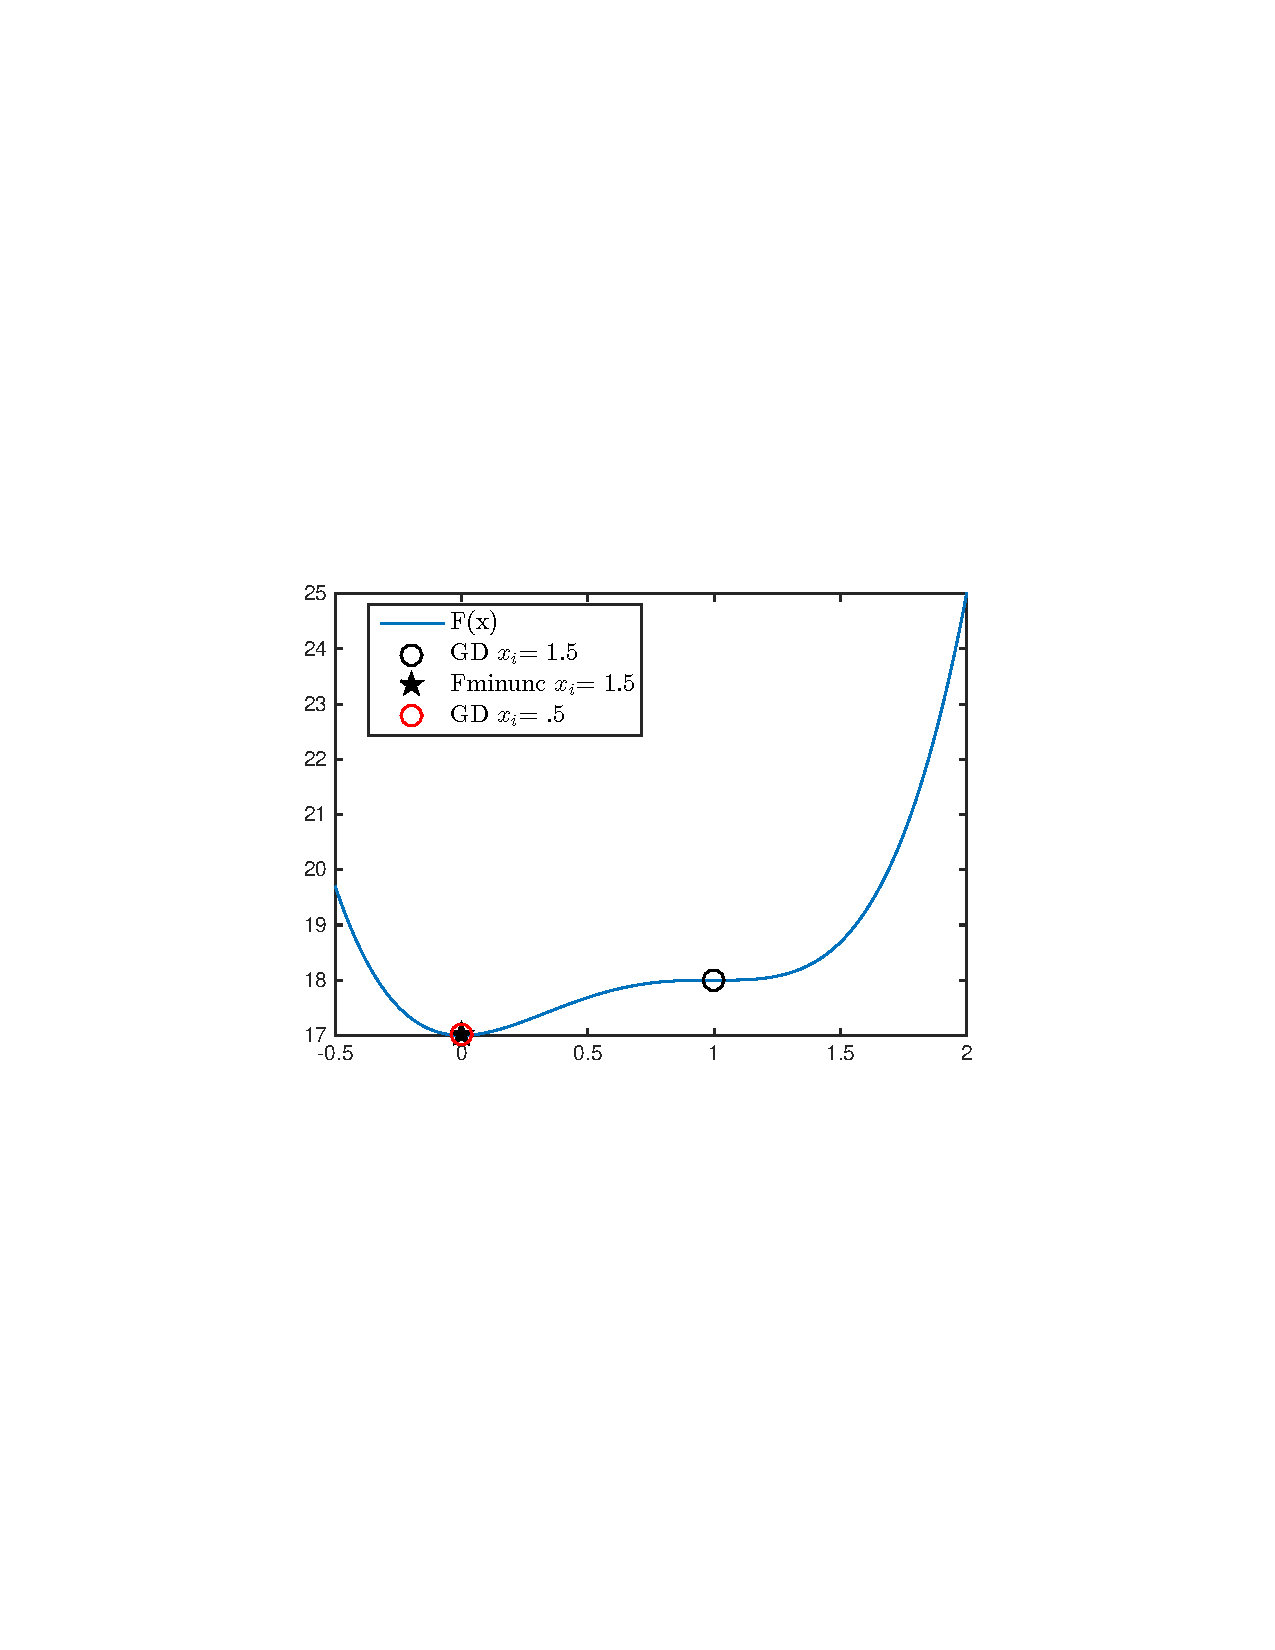
\includegraphics[scale =.6]{comparetofminunc.pdf}
\caption{Results of gradient descent algorithm versus results of fminunc for two initial guesses. For initial guess, $x_i= 1.5$ the gradient descent algorithm finds a local minimum but fminunc finds the global minimum}
\end{figure}
 

\begin{center}
  \begin{tabular}{ | c | c | c | c | c | }
    \hline
     function & $x_i$ & calls &  time (s) & global \\ \hline
     gradient descent & .5 &  11 &  0.009 & YES \\ \hline
     gradient descent & 1.5 & 1274  & 0.010 & NO \\ \hline
    fminunc & .5  & 6 & 0.022 & YES  \\ \hline
      fminunc &1.5 & 6 & 0.027 & YES \\ 
    \hline
  \end{tabular}
\end{center}
Depending on the starting guess, fminunc and our gradient descent algorithm sometimes differ even with the same tolerances applied. As shown in the above figure and table, fminunc is better than our gradient descent algorithm at finding the global minimum in the presence of local minima.  However, as fminunc takes more precise, and therefore fewer, steps,  it also requires more computation time .

\section{Linear Basis Function Regression}

\subsection*{Maximum Likelihood Weights}

The procedure for computing the maximum likelihood weights is as follows. First we must take the vector of inputs $x$ and compute the each individual basis vector, $\phi$, according to the definition given by the problem set, $\phi_1(x) = x, ... , \phi_M(x) = x^M$. Then we concatenate the basis vectors into a matrix $\Phi$. Finally, we can directly solve for the weight vector, $w$, using the formula $w_{ml} = (\Phi^T  \Phi)^{-1}  \Phi^T y$.

Shown below is a comparison of the weights we calculated versus the weights Bishop calculated for the same eight data points and different values of M and the corresponding graphs of the fit. Overall our results are nearly the same as those from the textbook.

\begin{table}
\begin{center}
	\begin{tabular}{| c | c | c | c | c |}
	\hline
	Source & M=0 & M=1 & M=3 & M=9 \\ \hline
	Computed  &  .19 & $\begin{bmatrix} .82 \\ -1.27 \end{bmatrix}$ & $\begin{bmatrix} .31 \\ 7.99 \\ -25.43 \\ 17.37 \end{bmatrix}$ & $\begin{bmatrix} .35 \\ \textcolor{red}{231.73} \\ \textcolor{red}{-5307.04} \\ \textcolor{red}{48435.64} \\  \textcolor{red}{-231018.45} \\ \textcolor{red}{638357.05} \\ \textcolor{red}{-1059050.39} \\ \textcolor{red}{1039740.82} \\ \textcolor{red}{-556279.81} \\ \textcolor{red}{124890.36} \end{bmatrix}$  \\ \hline
	Bishop  &  .19 & $\begin{bmatrix} .82 \\ -1.27 \end{bmatrix}$ & $\begin{bmatrix} .31 \\ 7.99 \\ -25.43 \\ 17.37 \end{bmatrix}$ & $\begin{bmatrix} .35 \\ 232.37 \\ -5321.83 \\ 48568.31 \\  -231639.30 \\ 640042.26 \\ -1061800.52 \\ 1042400.18 \\ -557682.99 \\ 125201.43 \end{bmatrix}$  \\ \hline
	\end{tabular}
\caption{Computed weights versus weights given in Bishop. Values in red show discrepancies.}
\end{center}
\end{table}

\begin{figure}[H]
\center
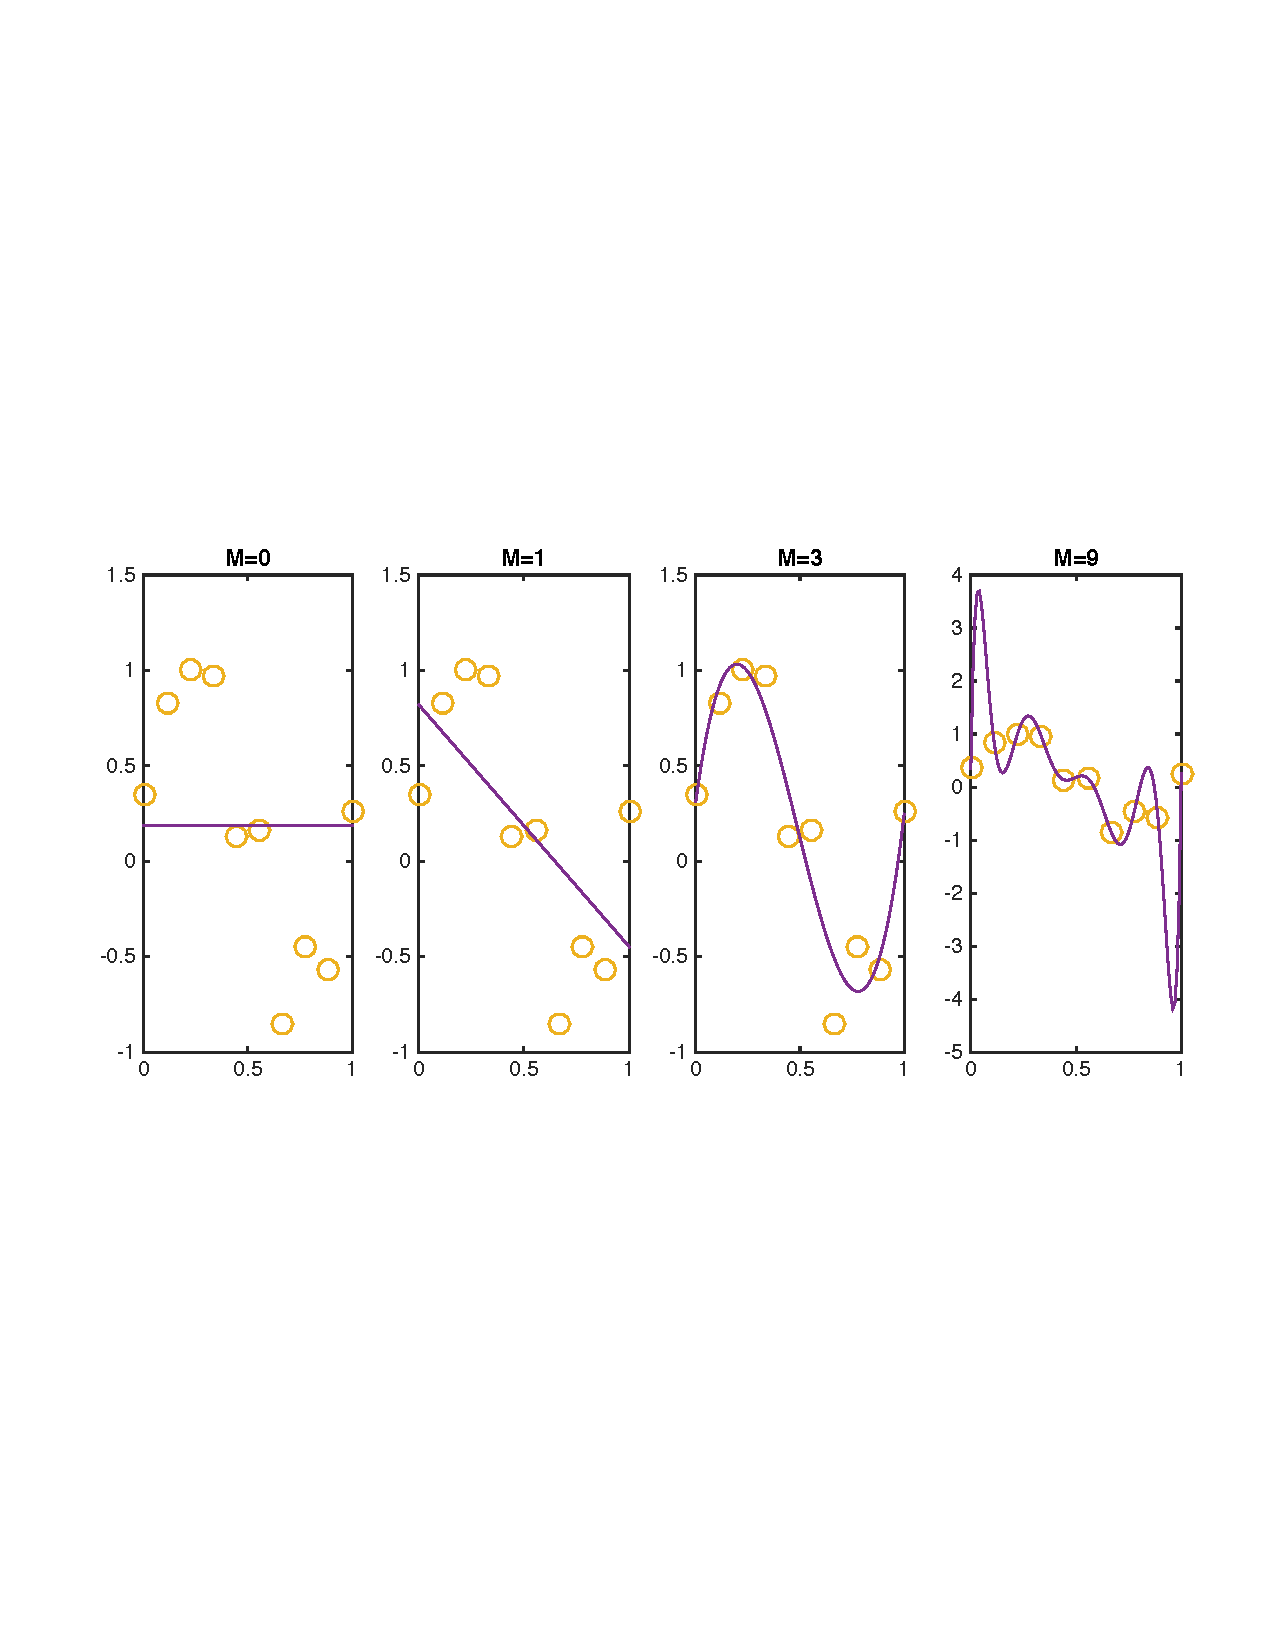
\includegraphics[scale =.45]{ML_weight.pdf}
\caption{Curves fit to data by maximum likelihood weights}
\end{figure}

\subsection*{ Sum of Squares Error}
For a particular hypothesis, $w, M $ and data points $(X, Y)$ the sum of squares error and its derivative are given by

\begin{align}
SSE(w) = (\Phi(M, X) w - Y)^T(\Phi(M, X) w - Y)\\
\frac{\partial SSE}{\partial w}= 2 \Phi(M,X)(\Phi(M,X)w -Y) 
\end{align}

The derivative was verified by testing against the numerical derivative code. Discrepancies for all tried values were under $10^{-10}$. 

For the same tolerances fminunc and the gradient descent algorithm found the same minimum. This is because the objective function is effectively a n-dimesion quadratic bowl so it has no issues with local minima. However, the gradient descent function takes significantly more function calls than fminunc. The exact number depends on the chosen step size and initial guess but can be many orders of magnitude larger. 

\subsection*{ Sine Basis Function}
If the basis functions were sine functions, it would fit this data set very well, just because the data was generated from a sine function. The weight for the $sin(2 \pi x)$ will be large, whereas the weights for the other larger frequency sine terms will be close to zero.

Had we not known the underlying distribution was itself a sine function, using sine functions for your basis functions can have two main potential disadvantages. First, it can require many terms to model simple functions (such as a line), and second not every function can be modeled only by sines, only odd functions can be modeled.

\section{Ridge Regression}

\subsection*{ Implementation}

To implement ridge regression a simple modification to the equation used in problem 2 was made
\begin{equation}
w_{ridge} = (\lambda I + \Phi^T  \Phi)^{-1}  \Phi^T y
\end{equation}

To compare to Bishop we implemented and plotted the results for $\lambda = {0, .1, .001} $

\begin{figure}[H]
\center
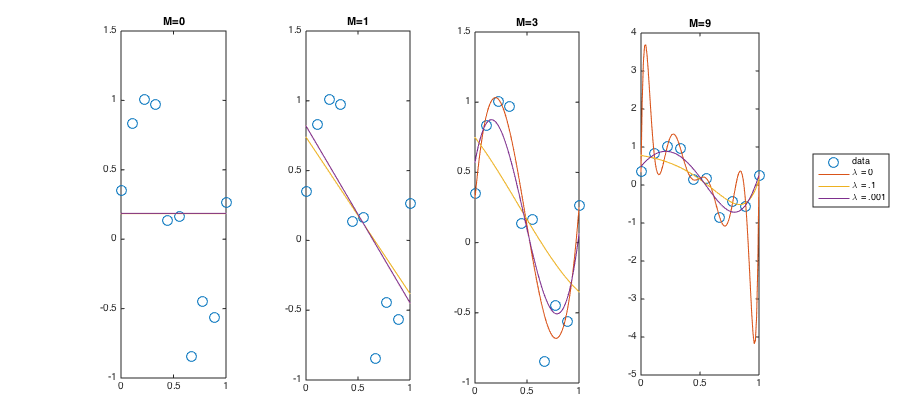
\includegraphics[scale =.3]{rr_lambdas.png}
\caption{Effect of $\lambda$ on data fit}
\end{figure}

recall that large $\lambda$ values penalize higher order terms. $\lambda = 0$ is the same as the maximum likelihood solution, so it is reasonable for lower order fits and overfitted when M is large. $\lambda = .1$ causes the polynomial to be too smooth, so the error to be very high. $\lambda = .001$ strikes a balance between too much error while still being generalizable. $\lambda = .001$ and M = 9 still produces a curve that looks similar to $sin(2\pi x)$, the function we originally sampled from.

\subsection*{ Model Selection}

\begin{figure}[H]
\center
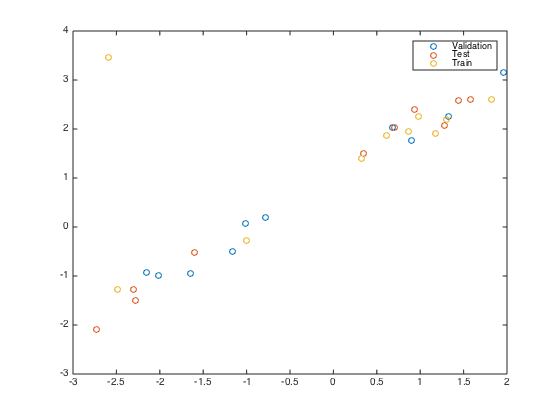
\includegraphics[scale =.3]{test_train_validate.png}
\caption{Provided data}
\end{figure}



Given the above training, test, and validation data, we ran a grid search optimization to find the best $\lambda$ and M for the ridge regression which minimized the sums of squares error. The minimum sum of squares error for the training data set occurred at M = 1 and $\lambda = 5$. These values also fit pretty well for the validation set, so we chose these parameters as our model selection. Below is the average performance of our model between the validation and test set.
 
\begin{table}
\begin{center}
  \begin{tabular}{ | c | c | c | c | c | }
    \hline
     $\lambda$ & M = 1 &  M = 2 & M = 3 \\ \hline
     0 & 17.55& 16.17 & 13.62  \\ \hline
     .1 & 17.36 & 16.16 & {13.57}  \\ \hline
     .2 & 17.17 & {16.16} & 13.58   \\ \hline
     .3 & 16.99 & 16.17 & 13.62   \\ \hline
     4 & 14.16 & 17.43 & 17.24   \\ \hline
     5 & \textcolor{red}{14.07} & 17.87 & 17.84  \\ \hline
     6 & 14.11 & 18.31 & 18.33  \\ \hline
    \hline
  \end{tabular}
  \caption{Average of the sum of squares error for the test and validation data sets. Model selection highlighted in red. }
\end{center}
\label{table:ave_sse}
\end{table}

As you can see in Table 2, there were other parameters (namely $\lambda = .1$ and M = 3) that would have performed better, but given only the training and validation sets, our chosen parameters performed well, achieving a 14.07 SSE. It makes intuitive sense that a good value for M would be 1, since the data seems to be drawn from something roughly linear.

\subsection*{ BlogFeedback Dataset}

\end{document}
